% !TEX root = ../main.tex
\subsection*{Addendum 5: Fiducial Cuts}
\addcontentsline{toc}{subsection}{Fiducial Cuts}
    % What are fiducial cuts.
    In detector physics, the fiducial region is defined as the region considered reliable and suitable for analysis.
    Fiducial cuts are constraints applied to experimental data in order to define this region.
    Thus, they allow us to exclude events or measurements that may be affected by experimental artifacts, detector inefficiencies, or other factors that could introduce systematic errors and biases \cite{leo1987}.

    % Why weren't fiducial cuts used in this thesis.
    Due to its 6-sector geometry, fiducial cuts are of particular importance for CLAS12 FD analysis.
    They were, however, disregarded for this particular analysis.
    This is because of the broadness of the study: we are only concerned with the phase space of DIS variables and the general statistics, as detailed in Section \ref{14.30::study_results}.
    While the cuts would likely improve the results, they are broad enough to be considered resilient to these improvements.

    % How would we implement them.
    To apply such cuts, we would need to follow the procedure described in \cite{zana2010}.
    This would involve providing $\phi$ vs $\theta$ curves that cuts all events at the edges of each DC sector.
    One curve would be needed for each $p$ bin, for each sector.
    Finally, different curves would be needed for each PID being processed.

    % Show plots.
    Examples of $\phi$ vs $\theta$ distributions for different $p$ bins can be seen in Figures \ref{fig::20.05::fiducial_cuts_pid11} and \ref{fig::20.05::fiducial_cuts_pid211}, where we show the distributions for $e^-$ and $\pi^+$.
    As can be seen on the plots, the separation between detector sensitive area and its edges is easily observed.

    % e-.
    \begin{figure}
        \centering
        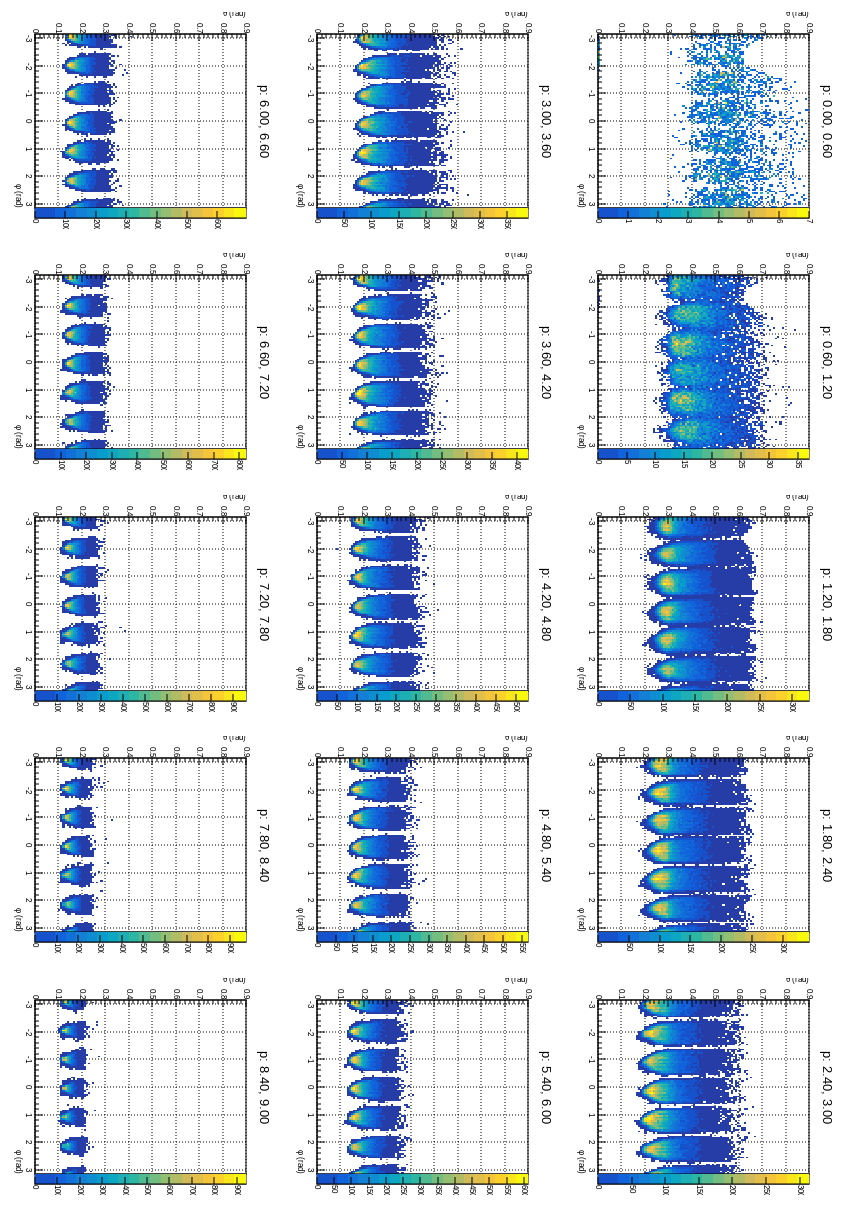
\includegraphics[width=\textwidth]{05fidcuts_11.png}
        \caption[$\phi$ vs $\theta$ of $e^-$ in $p$ bins]
        {$\phi$ vs $\theta$ of $e^-$ detected by DC, separated in $p$ bins.
        Run 12016.}
        \floatfoot{Source: Own elaboration, using the \href{https://github.com/bleaktwig/clas12-rge-analysis}{clas12-rge-analysis} software.}
        \label{fig::20.05::fiducial_cuts_pid11}
    \end{figure}

    % pi+.
    \begin{figure}
        \centering
        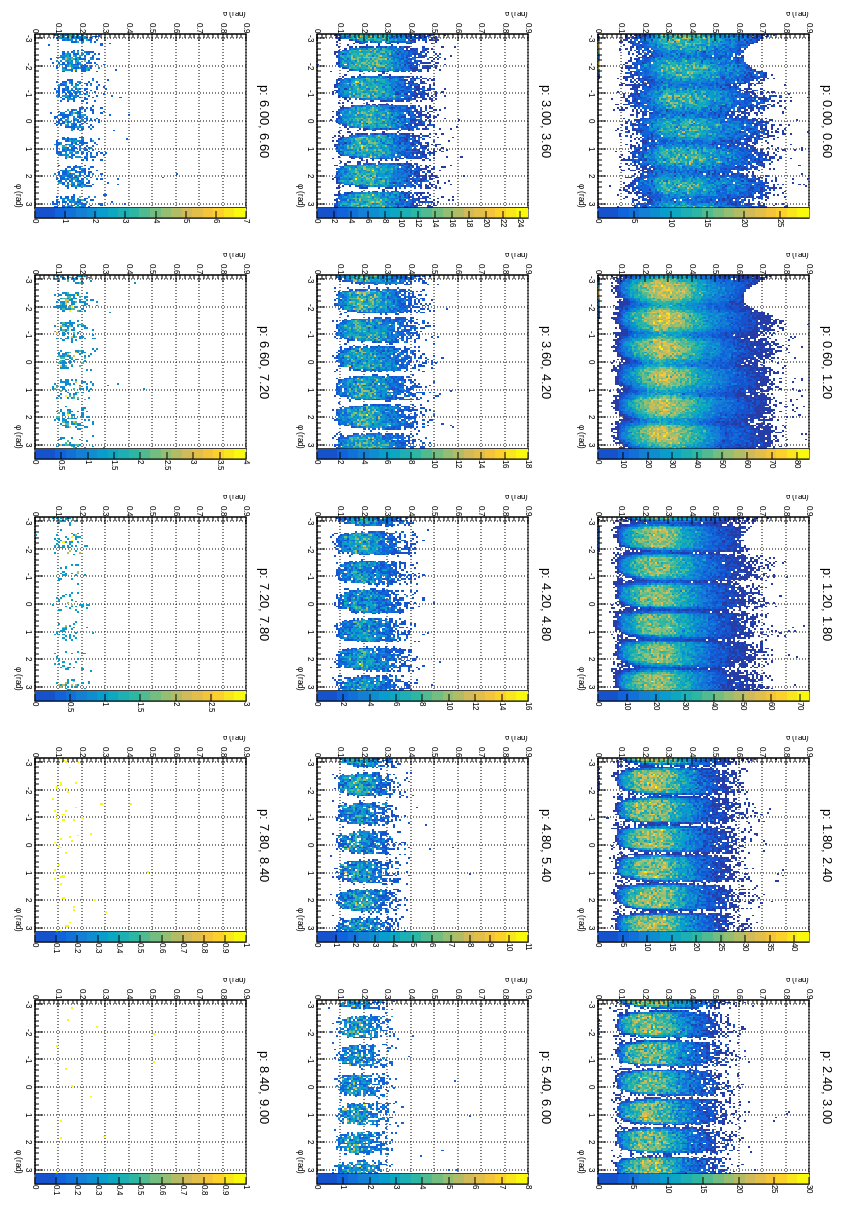
\includegraphics[width=\textwidth]{05fidcuts_211.png}
        \caption[$\phi$ vs $\theta$ of $\pi^+$ in $p$ bins]
        {$\phi$ vs $\theta$ of $\pi^+$ detected by DC, separated in $p$ bins.
        Run 12016.}
        \floatfoot{Source: Own elaboration, using the \href{https://github.com/bleaktwig/clas12-rge-analysis}{clas12-rge-analysis} software.}
        \label{fig::20.05::fiducial_cuts_pid211}
    \end{figure}
